\newpage
\chapter{Experiments and Results}
\label{sec:experiments}

Prior to jumping to the final results obtained with our algorithm, this chapter will attempt to give insight into the experiments we designed to verify our hypothesis. We examine our proposed methodology on two different but related scenarios. In the former scenario, we tackle the learning to count even hand-written digits, and for the latter one, crowd counting problem is considered. The findings of the experiments will determine to what extent synthetic data generation could help deep convolutional networks to learn when dealing with little amount of data. In addition, it will prove the applicability and scalability of DCNN as a well-suited substitute for feature detection problems. Hence, this chapter gives full particulars of each experiment, and presents obtained results as compared to similar works.

\section{Learning to Count Even-odd Handwritten Digits}

For our first objective, we intend to explore the features learned when training a deep CNN, in order to understand the underlying representations. In addition, we would like to examine the performance of the model in a larger scale compared to state-of-the-art approach \cite{segui2015learning}. To this end, we designed a synthetic problem of counting even digits in images. This experiment also helps illustrating the basic idea behind this work, where we hypothesize that the features learned during this task are:
\begin{enumerate}
\item Efficient descriptors of digits to enable the model to count them.
%\item Scaling up the task to examine if the same approach can be taken up for larger and more complex counting problems.
\item Sufficiently representative to be applied for the digit recognition tasks.  
\end{enumerate}

In this experiment, we feed images of digits into a deep convolutional neural network. Images are labeled with the number of even digits in each image. We took a regression analysis to tackle this problem. Therefore, the output of the network is a single number determining the model's prediction for the amount of even digits present in the images. 
 

\subsection{Dataset} 
As it was described in section ~\ref{subsubsec:digit}, we synthetically generated Even-odd digits dataset to use for this task. The dataset holds the following properties:
\begin{itemize}
\item Images of MNIST hand-written digits where each image contains up to 15 digits. Also the images are made in gray-scale.
\item Each image has a dimension of $100\times100$ and each digit in the image is $18\times18$ pixels.  
\item A minimum distance of 18 pixels is considered between each two digits (from center to center) in an image to prevent overlapping.
\item The dataset is generated uniformly. It means that there is an equal number of images for each amount of even digits in the image. For instance, the number of images with 5 even digits is the same as number of images containing 10 even digits.
\item The dataset of 1,000,000 samples is divided into a training set of 800,000 and a test set of 200,000 instances. 
\end{itemize}

Since we use Caffe platform to perform our experiments, we convert the images into LMDB format. LMDB uses memory-mapped files, so it has the read performance of a pure in-memory database while still offering the persistence of standard disk-based databases, and is only limited by the size of the virtual address space (it is not limited by the size of physical RAM). Therefore, we created two LMDB files for training and testing sets to be fed to the network.  

\subsection{Learning process}

As discussed in chapter~\ref{subsubsec:digitarch}, for learning to count the number of even digits, we designed a DCNN. Table~\ref{fig:digitnet} review the network's specification and architecture whereas table~\ref{hypar3} recaps the settings for the hyper-parameters.


\begin{table}[!htb]
    \begin{minipage}{.5\linewidth}
		\begin{table}[H]
			\centering
			\begin{tabular}{ |p{3.8cm}|p{1.7cm}| }
			\hline 
			\multicolumn{2}{|c|}{\textbf{Network hyper-parameters}} \\
			\hline
			\hline
			\textbf{Hyper-parameters} & \textbf{setting }\\
			\hline
			Learning rate & 0.0001\\
			\hline
			Learning policy    & \textit{Multi\_step} \\
			\hline
			step size   & 40000 \\
			\hline
			Momentum & $\mu = 0.9$\\
			\hline
			Weight decay & 0.0005 \\
			\hline
			Batch size & 256 \\
			\hline
			Iterations & 1000000 \\
			\hline
			\end{tabular}
				\caption{Proposed settings for network's hyper-parameters.}
				\label{hypar3}
		\end{table}
    \end{minipage}%
    \begin{minipage}{.5\linewidth}
		\begin{table}[H]
			\centering
			\begin{tabular}{ |p{2cm}|p{2cm}| }
			\hline 
			\multicolumn{2}{|c|}{\textbf{Network parameters}} \\
			\hline
			\hline
			\textbf{Layers} & \textbf{setting }\\
			\hline
			Conv1 & $20\times15\times15$\\
			\hline
			ReLU1 & max(x,0)  \\
			\hline
			LRN1 & $\alpha$=0.0001, $\beta$=0.75\\
			\hline
			Pool1    & $max(2\times2)$ \\
			\hline
			Conv2 & $50\times3\times3$\\
			\hline
			ReLU2 & max(x,0)  \\
			\hline
			LRN2 & $\alpha$=0.0001, $\beta$=0.75\\
			\hline
			Pool2    & $max(2\times2)$ \\
			\hline
			Conv3 & $50\times3\times3$\\
			\hline
			ReLU3 & max(x,0)  \\
			\hline
			LRN3 & $\alpha$=0.0001, $\beta$=0.75\\
			\hline			
			IP1 & 128 outputs \\
			\hline
			ReLU4 & max(x,0)  \\
			\hline
			IP2 & 64 outputs \\
			\hline
			ReLU5 & max(x,0)  \\
			\hline
			IP3 & 1 outputs \\
			\hline
			\end{tabular}
				\caption{Proposed architecture's settings.}
				\label{fig:digitnet}
		\end{table}
		 
    \end{minipage} 
        %\caption{Global caption}
\end{table}

%However, a well-designed network cannot solely guarantee an optimal performance for the model. The responsibilities of learning are divided between the network for yielding loss and gradients, and the optimization methods (solver) and parameters for overseeing the optimization and generating parameter updates. 

%Among Caffe solvers, As described in section~\ref{subsec:sgd}, we use Stochastic Gradient Descent optimization method. Apart from solver method, the solver parameters need to be set attentively in order to optimize the model performance. Table~\ref{tab:digitsolver} summarizes the initial settings for the solver parameters while the upcoming items justify our selections.

%\begin{table}[H]
%	\centering
%	\begin{tabular}{ |p{2cm}|p{2cm}| }
%	\hline 
%	\multicolumn{2}{|c|}{\textbf{Optimization parameters}} \\
%	\hline
%	\hline
%	\textbf{Parameter} & \textbf{value}\\
%	\hline
%	base\_lr & 0.0001\\
%	\hline
%	batch size & 256\\
%	\hline
%	momentum & 0.9  \\
%	\hline
%	weight decay & 0.0005\\
%	\hline
%	step size   & 40000 \\
%	\hline
%	gamma($\gamma$) & 0.1\\
%	\hline
%	iterations & 1,600,000\\
%	\hline
%	\end{tabular}
%		\caption{The solver parameters settings for even digit counting problem.}
%		\label{tab:digitsolver}
%\end{table}


%\begin{itemize}
%\label{solv:param}
%\item \textbf{Learning rate:} After trying different initial values in range of $(10^{-6}, 1)$, we set the basic learning rate to $\alpha = 0.0001$. However, for our experiment we chose \textit{multi-step} learning policy in which, after each \textit{stepsize}=40000 iterations, the learning rate drops by the rate of Gamma $\gamma = 0.1$. This initialization is based on rules of thumb used in \cite{krizhevsky2012imagenet}.
%\item \textbf{Batch size:} Due to the non-complex and low-resolution dataset we are training on, we were able to use batches of size 256 for our training and testing phases.
%\item \textbf{Momentum:} We use momentum $\mu = 0.9$. Because, momentum setting $\mu$ effectively multiplies the size of our updates by a factor of $\frac{1}{1-\mu}$. Hence, changes in momentum and learning rate ought to be accompanied with an inverse correlation. When momentum $\mu = 0.9$, we have an effective update size of 10 since we also drop the learning rate by the factor of $\gamma= 0.1$.
%\item \textbf{Weight decay:} Weight decay as a penalty term to the error function, has a constant value of 0.0005. This decay constant is multiplied to the sum of squared weights.
%\item \textbf{Iterations:} Given the time and hardware we had, we managed to let the system train for 1,600,000 iterations.
%\end{itemize}

\noindent The algorithm trained on a GPU NVIDIA \cite{kirk2007nvidia} Tesla K40 \cite{lindholm2008nvidia}. It took almost three days to train 800,000 samples and test over 200,000 images. Figure~\ref{fig:convha} illustrates the outputs (rectified responses of the shown filters) of the different layers in the network for one input sample. This illustration clearly depicts the process of even-digit counting in the proposed DCNN.  % The learning curves of this process are shown in the figure~\ref{fig:curve} (The shown graphs are shortened to the most inconstant (changing) section of the curves).

%\begin{figure*}[h!]
%    \centering
%    \begin{subfigure}[t]{0.5\textwidth}
%        \centering
%        {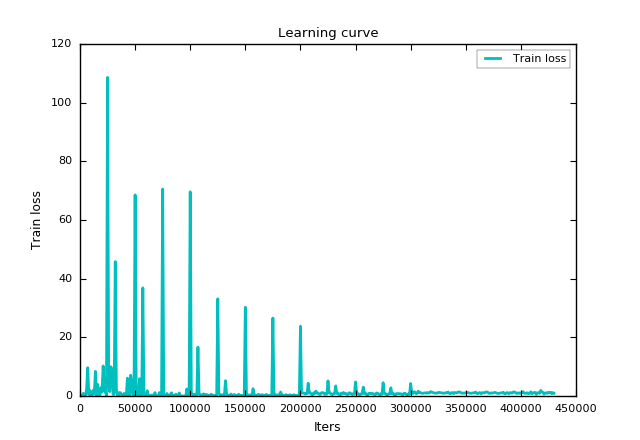
\includegraphics[width=1.1\textwidth]{images/ltc_train_real}}
%        \caption{Train loss.}
%    \end{subfigure}%
%    ~ 
%    \begin{subfigure}[t]{0.5\textwidth}
%        \centering
%        {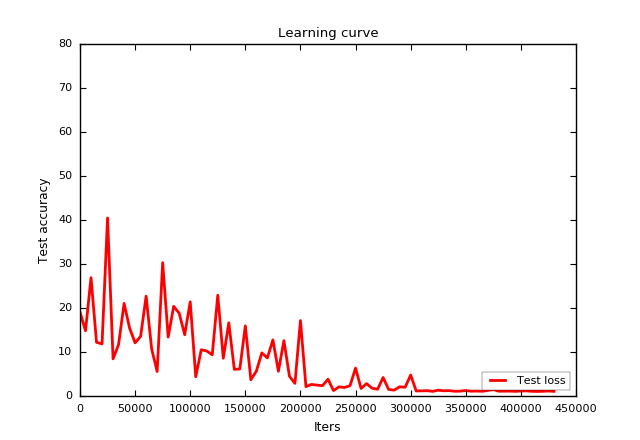
\includegraphics[width=1.1\textwidth]{images/ltc_test_real}}
%        \caption{Test loss.}
%    \end{subfigure}
%    \caption{Jagging cuts of learning curves of the model trained with even-digit dataset.}
%    \label{fig:curve}
%\end{figure*}
%
%As expected, the network learns without overfitting or underfitting. As you may notice, there is a sharp fall after each 100k iterations existing jagging in the figures which is due to the learning policy (\textit{step}) we chose for our experiment where we drop the learning rate after each 100000 iterations. We achieved \textbf{Train\_loss = 0.196} and consequently \textbf{Test\_loss = 0.213} on the test set.

%\noindent Moreover, figure~\ref{fig:convha} illustrates the outputs (rectified responses of the shown filters) of the different layers in the network for one input sample. This illustration clearly depicts the process of even-digit counting in the proposed DCNN. 

\begin{figure}[H]
	\centering
	{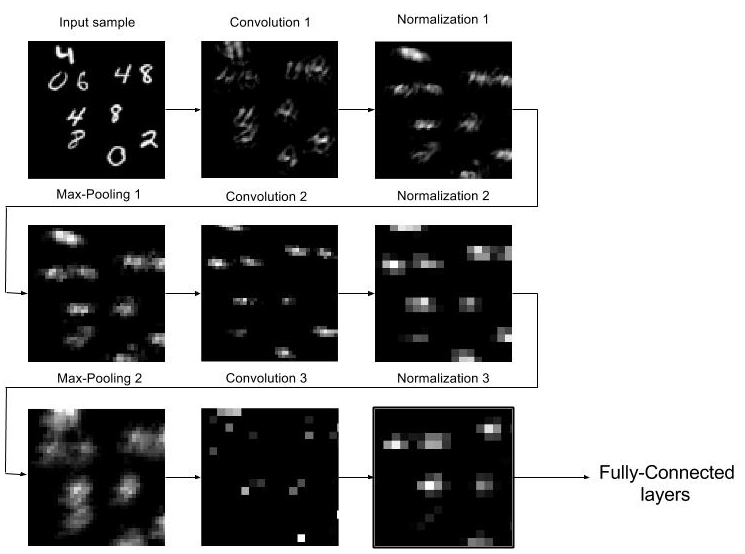
\includegraphics[width=0.8\textwidth]{images/mnist_convs}}
	\caption{Outputs of different layers an input image has been fed to. }
	\label{fig:convha}
\end{figure}

As you may see in the figures above, the main representations of the digits such as edges and general shape are successfully learned by the first convolutional layer. The second and third  convolutional layers provide more abstract information about the objects in the image. Although except for the first convolutional layer, the rest are not very interpretable for now, the activations correspondent to the digits' location can be seen. 




 

%Moreover, a schematic of the model with the output of each layer is depicted in figure~\ref{fig:digitnet}.
%%\begin{figure}[H]
%%	\centering
%	{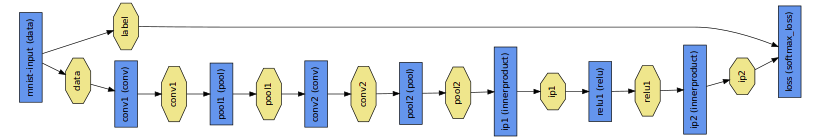
\includegraphics[width=1\textwidth]{images/caffe}}
%	\caption{An MNIST digit classification example of a Caffe network, where blue boxes represent layers and yellow octagons represent data blobs produced by or fed into the layers\cite{jia2014caffe}.}
%	\label{fig:digitnet}
%\end{figure}


\subsection{Experimental Results}
In addition to the Euclidean loss function that we implemented in our architecture, for comparison purposes, we introduce two other error measurements to evaluate and fairly compare the performance of our model with state-of-the-art solutions. These measurements are briefly described and justified in below:
%In addition to the Euclidean loss function that we implemented in our architecture, we need to use two other error measurements to evaluate and fairly compare the performance of our model with state-of-the-art solutions. These measurements are briefly described and justified in below:
\begin{enumerate}
\item \textbf{Mean squared error (MSE)}: Mean squared error is arguably the most important criterion used to evaluate the performance of a predictor or an estimator. The mean squared error is also useful to relay the concepts of bias, precision, and accuracy in statistical estimation. The MSE is the second moment (about the origin) of the error, and thus incorporates both the variance of the estimator and its bias \cite{lehmann1998theory}. The MSE can be estimated by
$$MSE = {\frac{1} {N}{\sum\limits_{i = 1}^N {(\hat{x_{pred}} - x_{obs} } })^{2} } $$
where:\\
\textit{N}: the number of instances\\
\textit{ $\hat{x_{pred}}$}: a vector of N predictions\\
\textit{$x_{obs}$}: a vector of observed value (ground truth) for input x\\

The mathematical benefits of mean squared error are particularly evident in its use for analyzing the performance of linear regression, as it allows one to partition the variation in a dataset into variation explained by the model and variation explained by randomness.
\item \textbf{Mean absolute error(MAE)}: MAE measures the average magnitude of the errors in a set of predictions, without considering their direction. In other words, it measures how close predictions are to the eventual outcomes \cite{willmott2005advantages}. MAE can simply be computed by:
$$MAE = {\frac{1} {N}{\sum\limits_{i = 1}^N {|x_{pred} - x_{obs} } }| } $$
where:\\
\textit{N}: number of instances\\
\textit{ $x_{pred}$}: prediction for instance x\\
\textit{$x_{obs}$}: observed value (ground truth) for instance x
\end{enumerate}

\noindent Having chosen error measurements explained, for the task of counting even digits, using 800,000 training samples and 200,000 test images, and after 1,600,000 iterations, our model obtained the results shown in table~\ref{tab:res}.


\begin{table}[H]
\centering
\small\sffamily
\begin{tabular}{llr}
%\toprule
\multicolumn{2}{c}{\textbf{\textbf{Counting Even-digits Results }}} \\
\bottomrule
\textbf{Error measurement}        & \textbf{Error} \\
\bottomrule
%\midrule
Euclidean loss           & 0.212  \\
Mean squared error       & 0.847  \\
Mean absolute error      & 0.394 \\
\bottomrule
\end{tabular}
\caption{}
\label{tab:res}
\end{table} 

Table above satisfactory results obtained from this learning process. Accordingly, the confusion matrix corresponding to the model is provided in figure~\ref{fig:splot} in below.

\begin{figure}[H]
	\centering
	{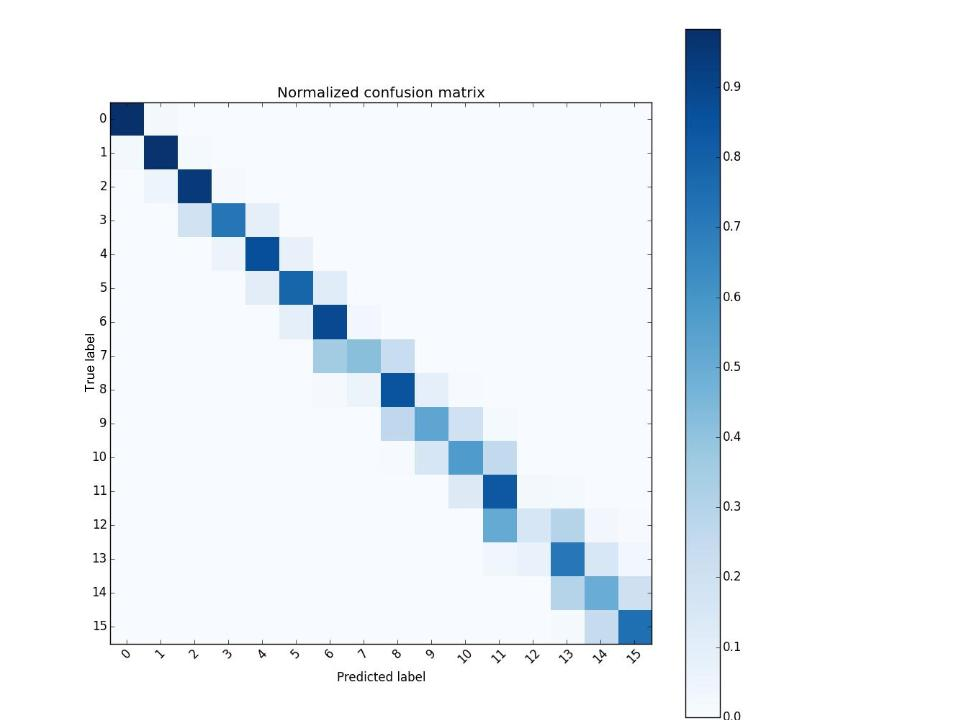
\includegraphics[width=0.9\textwidth]{images/normCM}}
	\caption{Normalized confusion matrix of the proposed model.}
	\label{conf}
\end{figure}


As you may observe in Figure~\ref{fig:splot}, most of the frames are correctly labeled. Moreover, most of the errors correspond to adjacent values. A similar experiment was done by \citeauthor*{segui2015learning}. In their work, they used images with up to 5 digits with different architecture. Also each digit in the images had a dimension of $28\times28$. They approached the problem as a classification task. 

%\indent Therefore, in order to provide a fair comparison, we calculated the accuracy in the same way as classification task (correct predictions/all test samples). Figure~\ref{conf} illustrates the confusion matrix obtained from this calculation. 
%%\begin{figure}[H]
%%	\centering
%%	{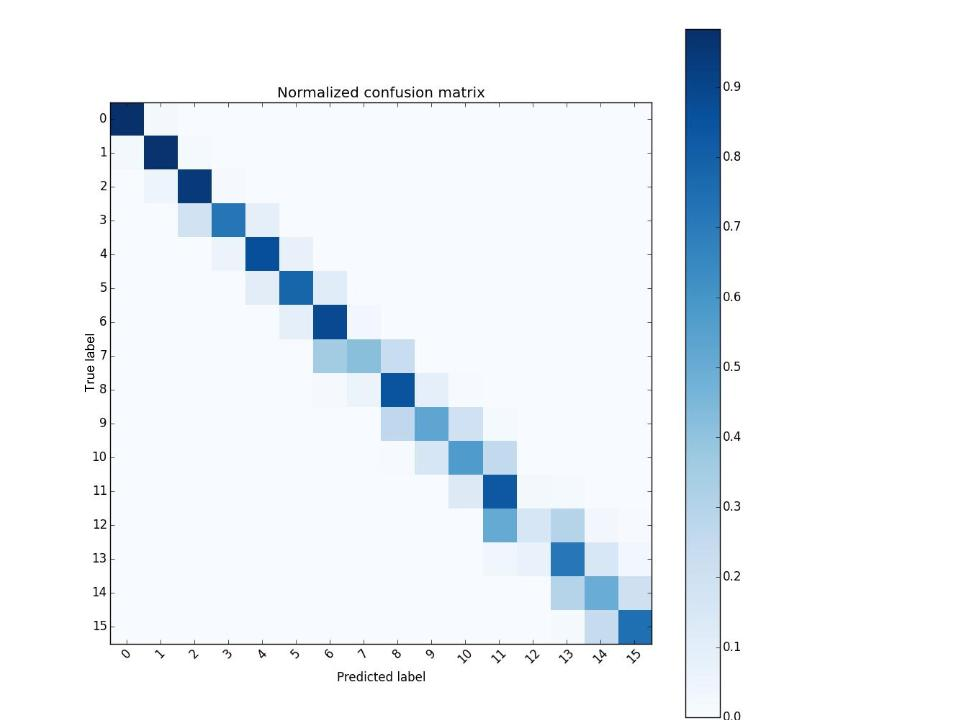
\includegraphics[width=0.9\textwidth]{images/normCM}}
%%	\caption{Normalized confusion matrix of the proposed model.}
%%	\label{conf}
%%\end{figure}

In order to demonstrate how far each model's accuracy stands from random, we provided randomness percentages according to each model. The following table~\ref{tab:comp} contrasts accuracy with pure chance values for each experiment. It is generally correct to say, that the model improves over the random.

% Moreover, we demonstrate how far each model's accuracy stands from random. These comparison has been shown in the table~\ref{tab:comp}.
%the difference the accuracy of both experiments from random, and from there we draw a proportional comparison.  These comparison has been shown in the table~\ref{tab:comp}.

\begin{table}[H]
\centering
\small\sffamily
\begin{tabular}{llr}
%\toprule
\multicolumn{3}{c}{\textbf{\textbf{Performance Comparison}}} \\
\bottomrule
\textbf{Experiments}  &   \textbf{Accuracy} & \textbf{Chance} \\
\bottomrule
%\midrule
Proposed architecture (up to 15 digits)     & 79.87\% & 6.25\% \\
\citet{segui2015learning} approach (up to 5)& 93.8\% & 16.66\%  \\

\bottomrule
\end{tabular}
\caption{Results comparison between our approach and state-of-the-art \cite{segui2015learning}.}
\label{tab:comp}
\end{table} 

As shown in the table above, considering the number of digits present in images and lower percentages of chance in our method, we obtained impressive results. However, due to different size and amount of digits in our dataset compared to state-of-the-art approach in \cite{segui2015learning}, it is not possible to draw a fair comparison between our work and state-of-the-art. We believe that by testing our model on a similar dataset to \citet{segui2015learning} approach, we would be able to achieve better results. However, since this experiment's focus is on analyzing scalability of DCNN application and also to introduce the basic idea behind this master thesis, we decided not to provide this comparison and be satisfied of achieving our main objectives.  

\subsection{Conclusion}

Noteworthy results obtained from the performance of designed model on the test set shows that not only DCNN are able to learn digits features, but also representativity of learned features can provide more scalability for the proposed problems. This fact assures us that the learned features are representative of digits to a high degree. This results show that DCNN are able to learn the object features incrementally and from the scratch without the need for any domain expert or feature descriptor methods. 

\section{Counting Pedestrians in a Walkway}

The first experiment proved that features can be learned from synthetically created datasets automatically using deep CNN. However, the use of deep architectures for fully supervised learning problems requires a large amount of annotated data. At the moment, for crowd counting problems, such data does not exist for research purposes. 

Hence, we propose a crowd counting problem using synthetic dataset in order to examine first, how well the model trained with synthetic images would perform. And then, whether the model is applicable for a real-world crowd counting scenario or not. We believe that this experiment will enlighten these questions. 

\subsection{Datasets} 

As fully discussed in chapter~\ref{subsec:synped}, for this particular case study, we synthetically created a dataset of 1 million images. To recap, the dataset specifications are the followings:
%\todo{no need to repeat the information, but i like the description of the dataset here better}, DONT UNDERSTAND WHAT YOU MEAN??!!!!
\begin{itemize}
\item Each image is in gray-scale, $158\times158$ pixels, normalized, and contains up to 29 pedestrians in a walkway. Images are labeled with the number of pedestrians present in the image.  
\item Pedestrians' location in the images are center-based. A mask (region of interest) has been applied to images that defines the area in which the pedestrians are counted. Thus, the person is labeled if it's center is put in the region of interest.   
\item Out of 1 million images, 800,000 are considered for training and 200,000 for testing sets.
\end{itemize} 

\noindent In addition, in order to examine the performance of our model in a real-world scenario, we used UCSD crowd counting dataset \cite{chan2008privacy} with the underneath properties:

\begin{itemize}
\item The dataset consists of 3375 video frames shot by a stationary camera. Each image has up to 29 pedestrians present in the image.
\item Images are in gray-scale, resized to $158\times158$ pixels, normalized (0 to 255) and filtered by the same mask (region of interest) as the other dataset. Labels are the number pedestrians placed in the region of interest.
\item Pedestrians annotation is center-based. The ones inside the mask are labeled.  
\item Images are continuous video frames of 20 different videos. Each video contains up to 200 images.  
\end{itemize}

Once again, to improve the training time, we converted the synthetic data into LMDB format for Caffe to read it in the fastest way.


\subsection{The Learning Process}

As fully described in chapter~\ref{subsec:ucsdarch}, we implemented a deep convolutional neural network in Caffe to learn the number of pedestrians in the walkway. As a reminder, the designed network has the components mentioned in table~\ref{myucsd3}. The network trains with stochastic gradient descent and our justification for the setting the solver parameters (hyper-parameters) remains the same as previous experiment (explained in section~\ref{subsec:ucsdarch}). However, once again table~\ref{hypar4} provides a review of the settings for network's hyper-parameters.

\begin{table}[H]
    \begin{minipage}{.5\linewidth}
		\begin{table}[H]
			\centering
			\begin{tabular}{ |p{2cm}|p{4cm}| }
			\hline 
			\multicolumn{2}{|c|}{\textbf{Network parameters}} \\
			\hline
			\hline
			\textbf{Layers} & \textbf{setting }\\
			\hline
			Conv1 & $10\times15\times15$\\
			\hline
			ReLU1 & max(x,0)  \\
			\hline
			LRN1  & $\alpha$=0.0001, $\beta$=0.75\\
			\hline
			Pool1 & $max(2\times2)$ \\
			\hline
			Conv2 & $10\times11\times11$\\
			\hline
			ReLU2 & max(x,0)  \\
			\hline
			LRN2  & $\alpha$=0.0001, $\beta$=0.75\\
			\hline
			Pool2 & $max(2\times2)$ \\
			\hline
			Conv3 & $20\times9\times9$\\
			\hline
			ReLU3 & max(x,0)  \\
			\hline
			LRN3  & $\alpha$=0.0001, $\beta$=0.75\\
			\hline
			
			Conv4 & $20\times5\times5$\\
			\hline
			ReLU4 & max(x,0)  \\
			\hline
			LRN4  & $\alpha$=0.0001, $\beta$=0.75\\
			\hline
			IP1   & 128 outputs \\
			\hline
			ReLU5 & max(x,0)  \\
			\hline
			IP2   & 64 outputs \\
			\hline
			ReLU6 & max(x,0)  \\
			\hline
			IP3   & 1 output \\
			\hline
			\end{tabular}
				\caption{Proposed architecture's settings.}
				\label{hypar4}
		\end{table}
    \end{minipage}%
    \begin{minipage}{.5\linewidth}
		\begin{table}[H]
			\centering
			\begin{tabular}{ |p{3.8cm}|p{1.7cm}| }
			\hline 
			\multicolumn{2}{|c|}{\textbf{Network hyper-parameters}} \\
			\hline
			\hline
			\textbf{Hyper-parameters} & \textbf{setting }\\
			\hline
			Learning rate & 0.0001\\
			\hline
			Learning policy    & \textit{Multi\_step} \\
			\hline
			step size   & 40000 \\
			\hline
			Momentum & $\mu = 0.9$\\
			\hline
			Weight decay & 0.0005 \\
			\hline
			Batch size & 256 \\
			\hline
			Iterations & 1600000 \\
			\hline
			\end{tabular}
				\caption{Proposed settings for network's hyper-parameters.}
				\label{myucsd3}
		\end{table}
    \end{minipage} 
        %\caption{Global caption}
\end{table}


%The model's optimization method and parameters (solver parameters) are set similar to the learning to count problem. The network trains with stochastic gradient descent and our justification for the setting the solver parameters remains the same previous experiment (explained in section~\ref{solv:param}). Therefore, the repetitive explanations are skipped and only the final settings are described in table~\ref{tab:solvparam}.

%\begin{table}[H]
%	\centering
%			\caption{The solver parameters settings for even digit counting problem.}
%	\begin{tabular}{ |p{2cm}|p{2cm}| }
%	\hline 
%	\multicolumn{2}{|c|}{\textbf{Optimization parameters}} \\
%	\hline
%	\hline
%	\textbf{Parameter} & \textbf{value}\\
%	\hline
%	base\_lr & 0.0001\\
%	\hline
%	batch size & 256\\
%	\hline
%	momentum & 0.9  \\
%	\hline
%	weight decay & 0.0005\\
%	\hline
%	step size   & 40000 \\
%	\hline
%	gamma($\gamma$) & 0.1\\
%	\hline
%	iterations & 1,600,000\\
%	\hline
%	\end{tabular}
%
%		\label{tab:solvparam}
%\end{table}

\noindent Similarly, we used GPU NVIDIA TESLA K40 to train our network. After 5 days of training, we obtained the following learning curves (figure~\ref{fig:ucurve}) :

\begin{figure*}[h!]
    \centering
    \begin{subfigure}[H]{0.5\textwidth}
        \centering
        {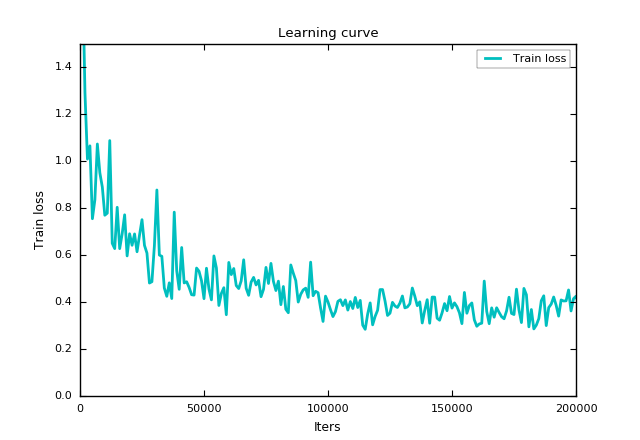
\includegraphics[width=1\textwidth]{images/train_U}}
        \caption{Training loss. }
    \end{subfigure}%
    ~ 
    \begin{subfigure}[H]{0.5\textwidth}
        \centering
        {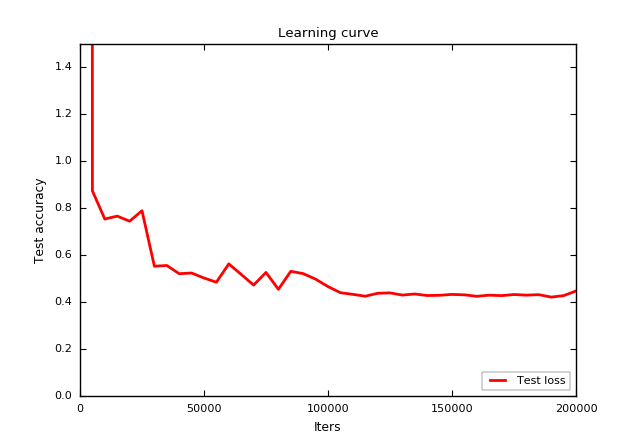
\includegraphics[width=1\textwidth]{images/test_U}}
        \caption{Test loss.}
    \end{subfigure}
    \caption{Inconstant snips of Learning curves of the model trained with synthetic dataset. }
    \label{fig:ucurve}
\end{figure*}





As you may observe, the correspondent decreasing of training and test loss clearly proves that the network has neither over-fitted nor under-fitted. We achieved \textbf{Train loss = 0.425065} and consequently \textbf{Test loss = 0.447545} on the test set.

\noindent The network was able to learn sufficient features corresponding to the pedestrians. To illustrate, the outputs for one input sample, after each layer in the network, has been depicted in the following figures~\ref{fig:feats}: 



\begin{figure}[H]
	\centering
	{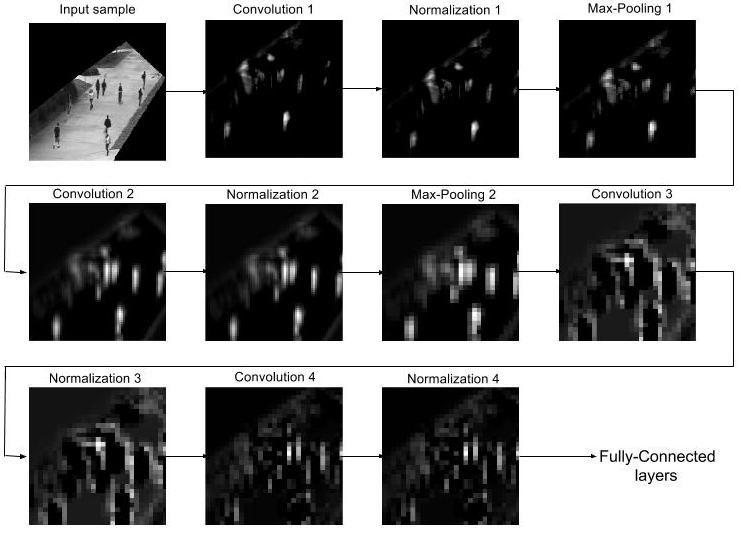
\includegraphics[width=0.9\textwidth]{images/ped_convs}}
	\caption{The outputs of each layer in the network for one data sample. }
	\label{fig:feats}
\end{figure}



Similar to the previous experiment, the first convolutional layer provides us with the most important and illustrative information about the pedestrians we aim to count. As you may notice, mostly the first two convolution layers have successfully detected the pedestrians contours in the image. The size of kernels in convolutional layers helps improving this detection. We intended to avoid learning too much details (noise) by choosing kernel sizes of first two convolutional layers relatively large. In this way, the network ignores the details that would not help detecting pedestrians in the images. 

\subsection{Experimental Results}

Equivalently to the first analysis, we use mean squared error, mean absolute error and the default euclidean loss function to present the results obtained in this experiment. Having that said, the following results were obtained:

\begin{table}[H]
\centering
\small\sffamily
\begin{tabular}{llr}
%\toprule
\multicolumn{2}{c}{\textbf{\textbf{Synthetic Crowd Counting Results}}} \\
\bottomrule
\textbf{Error measurement}        & \textbf{Error} \\
\bottomrule
%\midrule
Euclidean loss           & 0.447545  \\
Mean squared error       & 0.942795  \\
Mean absolute error      & 0.707661  \\
\bottomrule
\end{tabular}
\caption{.}
\label{tab:res}
\end{table} 

Considering the random percentage (0.033) of this experiment, the network shows a remarkable performance on counting the number of pedestrians. These results were attained after 1,600,000 iterations on 800,000 train and 200,000 test sets. Correspondingly, figure~\ref{fig:splot} depicts the spread-error plot of the model performance on the test set.

\begin{figure}[H]
	\centering
	{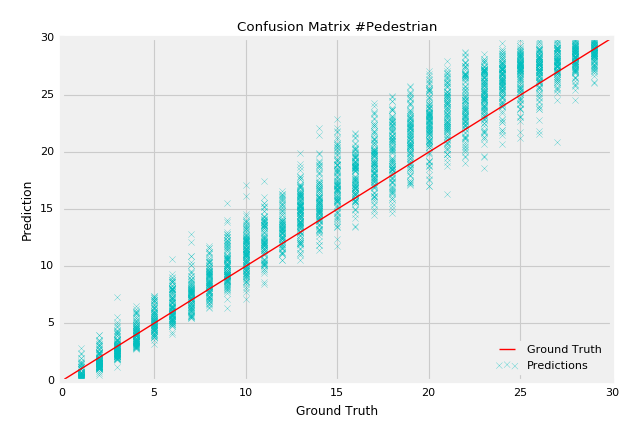
\includegraphics[width=0.8\textwidth]{images/syntheticGraph}}
	\caption{Confusion matrix regarding the model trained on the synthetic dataset.}
	\label{fig:splot}
\end{figure}

As you may notice, the network's predictions closely follow the target values. Also a direct correlation between the number of pedestrians and error deviation can be inferred from the plot which is reasonable due to the more overlapping in the crowded scenes. 

\noindent In state-of-the-art, \citet{segui2015learning} did a similar experiment with maximum 25 pedestrians in each image. In addition, the difference between their work and our analysis, mainly revolves around the synthetic data generation algorithm and the designed architectures. Nonetheless, the table of comparison between these two approaches are shown in below:
 
\begin{table}[H]
\centering
\small\sffamily
\begin{tabular}{llrr}
%\toprule
\multicolumn{4}{c}{\textbf{\textbf{Performance Comparison}}} \\
\bottomrule
\textbf{Experiments} &\textbf{MSE} &\textbf{MAE}& \textbf{Chance} \\
\bottomrule
%\midrule
Our approach (29 pedestrians)                  & \textbf{0.942}   &  \textbf{0.707}        & 3.33\% \\
\citet{segui2015learning} (25 pedestrians)     & 1.12       & 0.74     & 4.00\% \\
\bottomrule
\end{tabular}
\caption{Comparison between our results and state-of-the-art. As you may observe, although we there are more pedestrians in our images, our model shows a more promising performance.  }
\label{tab:tab}
\end{table} 

Table~\ref{tab:tab} shows that even though our synthetic dataset contains more pedestrians in images, the model predicts the multiplicity of pedestrians more accurate than state-of-the-art \cite{segui2015learning}. This improvement validates the benefit of introduced synthetic data and defined architecture for this task. 

%\noindent As an innovative part of this Master thesis, we were interested to figure out if we have been able to overcome the exhaustive labeling in real problems such as crowd counting. For this reason, we tested our model on a real UCSD crowd counting dataset \cite{chan2008privacy}.
\noindent Furthermore, as an innovative part of this Master thesis, we were interested in figuring out if we have been able to overcome the exhaustive labeling in real problems such as crowd counting by testing our model on real-world UCSD crowd counting dataset collected by \citet{chan2008privacy}. Having our model tested on UCSD real dataset of 3375 images, we obtained the results shown in table~\ref{tab:ucsdreal}:

% % % % % %DISCUSSION % % % % % % %
% In order to do that, we tried to minimize the difference (Euclidean) between training images and real images by adding a gaussian filter to the real images. We compared the predictions and true labels for $\sigma \in (0,2)$ to find the best sigma $\sigma$ value for filtering the real images. Figure~\ref{sigsig} depicts this process: 
%
%
%\begin{figure}[H]
%	\centering
%	{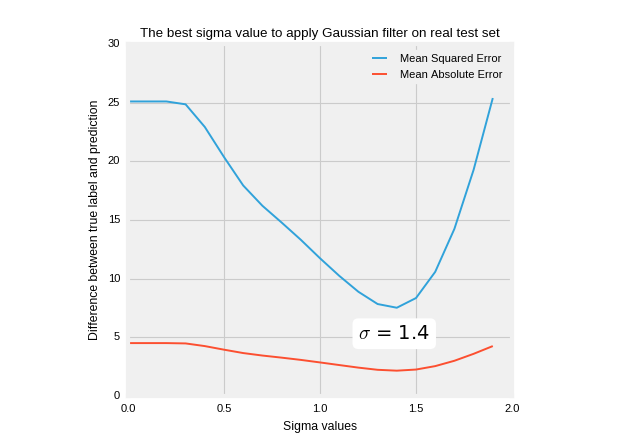
\includegraphics[width=0.8\textwidth]{images/sigmaTest}}
%	\caption{The best sigma value for the gaussian filter applied on real images.}
%	\label{sigsig}
%\end{figure}
%
%Setting the sigma value to $\sigma = 1.4$, table~\ref{tab:ucsdreal} demonstrates the performance of our model on UCSD dataset.

\begin{table}[H]
\centering
\small\sffamily
\begin{tabular}{llr}
%\toprule
\multicolumn{2}{c}{\textbf{\textbf{Real Crowd Counting Results}}} \\
\bottomrule
\textbf{Error measurement}        & \textbf{Error} \\
\bottomrule
%\midrule
Mean squared error       & 3.61  \\
Mean absolute error      & 1.38  \\
\bottomrule
\end{tabular}
\caption{The obtained results from testing our model on UCSD pedestrian dataset \cite{chan2008privacy}. }
\label{tab:ucsdreal}
\end{table} 

As it can be inferred from the above table, the results are convincing and rational given the results we achieved on the synthetic test set and the inevitable differences between the synthetic and real datasets. A confusion matrix regarding this experiment is shown in figure~\ref{confnew2}. We believe that this difference is mainly due to the difference between train and test images that can be handled by either modifying the architecture in a way to ignore more details, or improving the train set to become closer to the real test images. 

\begin{figure}[H]
	\centering
	{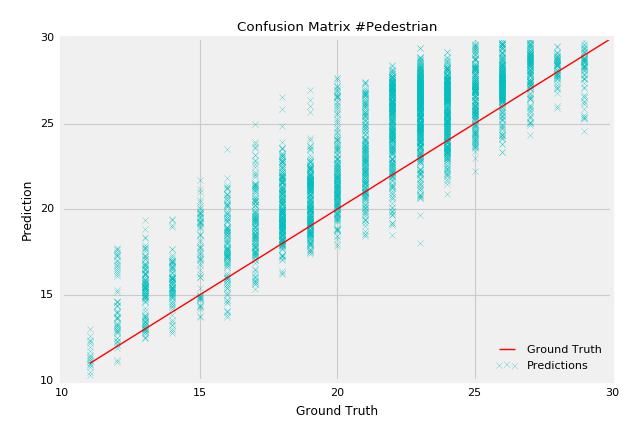
\includegraphics[width=0.8\textwidth]{images/realtestfig}}
	\caption{Confusion matrix regarding the model performance on the real test set. The starting point of the graph is 10 since the minimum amount of pedestrians in the real test set is 10.}
	\label{confnew2}
\end{figure}
The figure above shows that the model mostly over-predicts. This means that most probably sue to the inevitable differences between real and synthetic samples, the model is detecting some unseen noises as pedestrians. As you observe in the figure~\ref{confnew}, as the number of pedestrians increases in the images, the prediction accuracy of the model decreases.  


\noindent Moreover, we compared our model with \citeauthor*{chan2008privacy} research study in \cite{chan2008privacy} regarding crowd counting using exhaustive labeling and hand-crafted feature detectors using UCSD dataset. One difference we need to mention is that in their work, since the feature detection process was highly specialized for that particular problem, they computed the results for pedestrians towards camera and away from camera separately. However, in our dataset, we consider all pedestrians as one group of objects. Hence, we compare the average results of people towards and away from camera with our results. This comparison has been drawn in the following table~\ref{finalres}:

\begin{table}[H]
\centering
\small\sffamily
\begin{tabular}{llrr}
%\toprule
\multicolumn{3}{c}{\textbf{\textbf{Performance Comparison}}} \\
\bottomrule
\textbf{Experiments} &\textbf{MSE} &\textbf{MAE} \\
\bottomrule
%\midrule
Proposed method                  &  3.61 & 1.38      \\
\citet{chan2008privacy} approach &  2.73 & 1.24      \\
\bottomrule
\end{tabular}
\caption{Comparison between our results and real-world state-of-the-art approach done by \citet{chan2008privacy}.}
\label{finalres}
\end{table} 

 Although our synthetic images look highly realistic, still there are some undeniable differences between synthetic and real images. We believe that this difference is the main reason that hindered our proposed model to out perform state-of-the-art approach in \cite{chan2008privacy}. However, the attained results are not far away from the cutting-edge solutions.
 
\subsubsection{Discussions}

Regarding the results and analysis we did on real UCSD dataset, we attempted to minimize the difference (Euclidean distance) between synthetic and real images. In order to do that, we tried two approaches explained underneath. 

As the first endeavor, we applied a gaussian filter on the real test set. To do so, we needed to find the sigma value (standard deviation) which minimizes the euclidean distance between images. Therefore, we selected a validation set of 100 images from the real dataset along with 100 synthetic images. By calculating the image-wise euclidean distance between synthetic and real images for sigma $ \sigma \in (0, 2) $, we obtained the best sigma value as $ \sigma = 1.4 $. Figure~\ref{sigsig} demonstrates this process. 
\begin{figure}[H]
	\centering
	{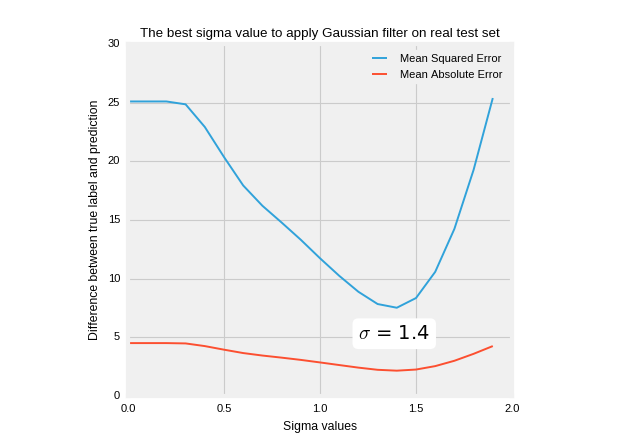
\includegraphics[width=0.8\textwidth]{images/sigmaTest}}
	\caption{The best sigma value for the gaussian filter applied on real images.}
	\label{sigsig}
\end{figure}
By testing our model on the test set images filtered with $ \sigma=1.4 $, we could not improve the results. Therefore we decided to make synthetic images filtered in order to minimize their euclidean distance to the real images. Therefore, we took up the same approach but this time for synthetic image. We obtained the best sigma value as $ \sigma=1.6 $ for the gaussian filter to blur the synthetic images as it is illustrated in figure~\ref{sig2}.   
\begin{figure}[H]
	\centering
	{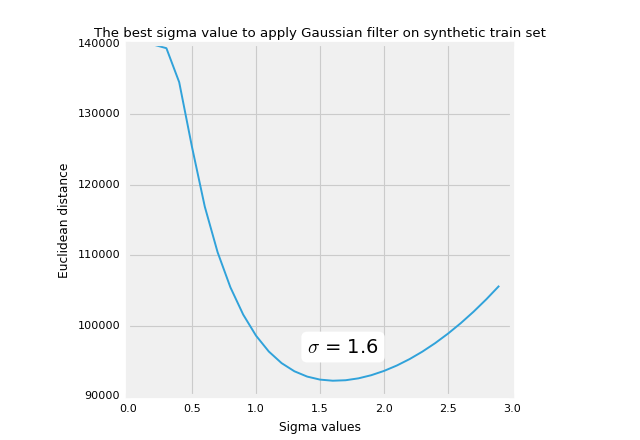
\includegraphics[width=0.8\textwidth]{images/sigmaTrain}}
	\caption{The best sigma value for the gaussian filter applied on real images.}
	\label{sig2}
\end{figure}
However, despite the fact that it improved the results to some extent, the improvement was not significant. Hence, we decided not to include this process in our main experiment. 
% adding a gaussian filter to the real images. We compared the predictions and true labels for $\sigma \in (0,2)$ to find the best sigma $\sigma$ value for filtering the real images. Figure~\ref{sigsig} depicts this process: 
%
%
%\begin{figure}[H]
%	\centering
%	{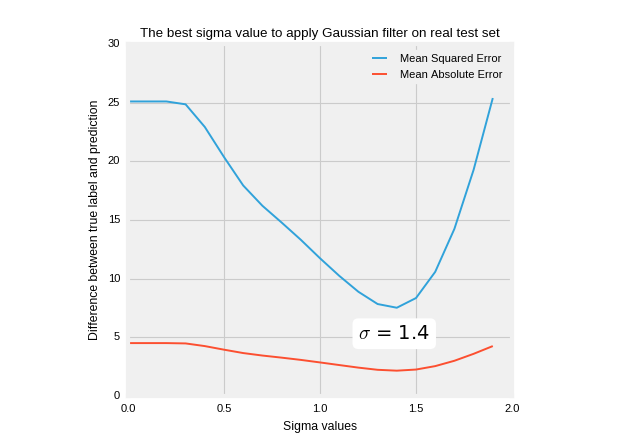
\includegraphics[width=0.8\textwidth]{images/sigmaTest}}
%	\caption{The best sigma value for the gaussian filter applied on real images.}
%	\label{sigsig}
%\end{figure}
%
%Setting the sigma value to $\sigma = 1.4$, table~\ref{tab:ucsdreal} demonstrates the performance of our model on UCSD dataset.

\subsection{Conclusion}

This experiment justifies our hypothesis regarding first, the benefit of generation and incorporation of synthetic datasets for learning via DCNN. Beside obtaining impressive results on the synthetic test set, we could improve the state-of-the-art results on the synthetic dataset obtained by \citet{segui2015learning}, while having more pedestrians in our images. This improvement implies the relative success of our synthetic data generation algorithm and architecture design.

Furthermore, although we were not able to improve the state-of-the-art solutions on the real pedestrian dataset, we were able to obtain noticeable results as well as facilitating the data annotation by using synthetic dataset for training the model. In addition, taking up DCNN approach, we alleviated feature detection efforts to a great extent. 
